\section{Factors That Correlate to Pursuit of Nuclear Weapons}
\label{s_factors}

Social science literature has suggested that a variety of political and technical factors that may motivate a state to pursue nuclear weapons. Political factors include: degree to which governing structure is authoritarian versus democratic, level of military spending, degree to which state is isolated militarily, level of conflict with other states. Technical factors include: degree to which the state's scientific expertise is integrated into the international community, nuclear reactor experience, indigenous reserves of natural uraniaum, and the ability to enrich uranium.  \TODO{Citations for why each factor was chosen.}

We have compiled a database of information that quantifies each of these eight factors for states at important historical points. This database is publically accessable at \TODO{link GITHUB}, and complete documentation on source data and assumptions is available at \TODO{link README}.  The set includes 42 unique states that have historically had either nuclear energy or weapons technology.  The 24 states that have never pursued weapons have data compiled for 2015. The 19 states that have pursued weapons at some point in the past have data for the year in which they pursued as well as the year in which they acquired a weapon, if applicable. Pursuit and acquisition dates are coded from \TODO{CITE}.  \TODO{Singh and Way} define pursuit date as the first year in which a significant decision to pursue nuclear weapons was made such as a political decision by cabinet-level officials, movement toward weaponization, or development of single-use, dedicated technology.  Acquire date indicates the year in which either the first explosion of a nuclear device occurred or the complete assembly of a weapon since not all countries tested their nuclear weapons.

\begin{table}
\centering
\begin{tabular}{|c|c|}
\hline
\textbf{Factor}        & \textbf{Source Database} \\
\hline
Authoritarian            & Center for Systemic Peace \\
                          & Polity IV Annual Time-Series, 1800-2015\cite{polity_scores}\\
\hline
Military Spending & SIPRI Military Expenditure Database 1949–2015\TODO{cite https://www.sipri.org/databases/milex} \\
\hline
Military Isolation & ???\TODO{Fill in and cite} \\
\hline
Conflict & ?????\TODO{Fill in and cite} \\
\hline
Scientific Network     & Internal Expert Opinion considering GDP, opportunities for scientists to study abroad \\
 & nuclear infrastructure, technical human capital \\
\hline
Nuclear Reactors           &  IAEA Power Reactor Database \TODO{ https://www.iaea.org/PRIS/CountryStatistics/CountryStatisticsLandingPage.aspx}\\
                         & IAEA Research Reactor Database \TODO{https://nucleus.iaea.org/RRDB/RR/ReactorSearch.aspx?rf=1}   \\
 \\
\hline
Enrichment/Reprocessing   & Nuclear Latency Dataset \TODO{Fuhrmann, M. and Tkach, B. (2015)}
\\
\hline
Uranium Reserves  &    OECD Uranium: Resources, Production and Demand Report \TODO{https://www.oecd-nea.org/ndd/pubs/2014/7209-uranium-2014.pdf}
 \\
\hline
\end{tabular}
\caption{Source data for each factor contributing to pursuit of nuclear weapons addressed in this paper.\TODO{SYSTEMIC PEACE HAS COPYRIGHT RESTRICTIONS}}
\label{tab:factor_sources}
\end{table}

\subsection{Pursuit Score}\label{s_pe}
The source used to define each factor has been taken from social science literature and is listed in table \ref{table:factor_sources} The raw data for each attribute has been normalized on a 1-10 scale so that all factors can be compared directly, as described in Appendix \ref{s_appendix}. The conflict requires a special note. Conflict has been defined historically for a given state by identifying three significant state-pair relationships.  Each of these relationships is coded as enemy, neutral, or ally.  Each of the two states in the pair is also identified as being a non-weapons state, known to be pursuing weapons, or a weapons-state.  The combination of weapons status and relationship status is combined to provide a conflict score for each pair. The net conflict factor is the average of the state's three conflict scores.

Once every state had been assigned a 0-10 score for each factor, a correlation
analysis was applied to the derived factor scores to quantify the degree to
which each individual factor is correlated to the decision whether or not to
pursue weapons. 
Each weight factor corresponds the Pearson correlation coefficient, or
the bivariate correlation between the factor and the score and can be
determined using the equation \ref{eqn:correlation}:
\begin{equation}
    \label{eqn:correlation}
    w_{f} = \frac{\sum_{i=0}^{N} (f_{i} - \bar{f}) (s_{i} - \bar{s})}
                 {\sqrt{\sum_{i=0}^{N}\left(f_{i} - \bar{f}\right)}
                 \sqrt{\sum_{i=0}^{N}\left(s_{i} - \bar{s}\right)}},
\end{equation}
where $N$ corresponds to the number of countries, $f_{i}$ and $s_{i}$ respectively
to the factor and the score of the country $i$ and, $\bar{f}$ and $\bar{s}$ to
the mean factor and the mean score over all the countries.

The final pursuit score is defined as the weighted linear combination of
its different factors. The final pursuit score has been normalized to have
values distributed between 0 and 10.

\TODO{ADD DETAILS OF HOW THE CORRELATION ANALYSIS WAS DONE.
Something about ordered results for pursue vs not-pursue. Final pursuit score
defined as a weighted linear combination of the factors}.  


\begin{table}
\centering
\begin{tabular}{|c|c|}
\hline
\textbf{Factor}        & \textbf{Weight} \\
\hline
Authoritarian   & 0.12 \\
Military Isolation & 0.075 \\
Reactors           & -0.18 \\
Enrichment \& Reprocessing & 0.10 \\
Scientific Network & 0.05 \\
Military Spending & 0.21 \\
Conflict  & 0.26 \\
Uranium Reserves &  0.0 \\
\hline
\end{tabular}
\caption{Relative weighting of each factor toward pursuit decision as determined by correlation analysis of historical data. Note reactor technology is anti-correlated.}
\label{tab:factor_weights}
\end{table}

The relative weights of the 8 factors are shown in \ref{table:factor_weights}.  Two major insights arise from this analysis. Firstly, a state's reactor technology is anti-correlated to pursuing a nuclear weapon.  Denoted in the table with a minus sign for illustrative purposes, in practice the factor scale was inverted such that maximum reactors led to a minimum reactor score, and then the absolute value of the weight (18\%) was used.  Secondly, indigenous uranium reserves were uncorrelated to weapons programs. These two results were not predicted by the social science literature.



\iffalse
% Google spreadsheet: CVT_Research/Collaborations/Fuel Cycle Facility Signatures
\begin{figure}%[htbp!]
\begin{center}
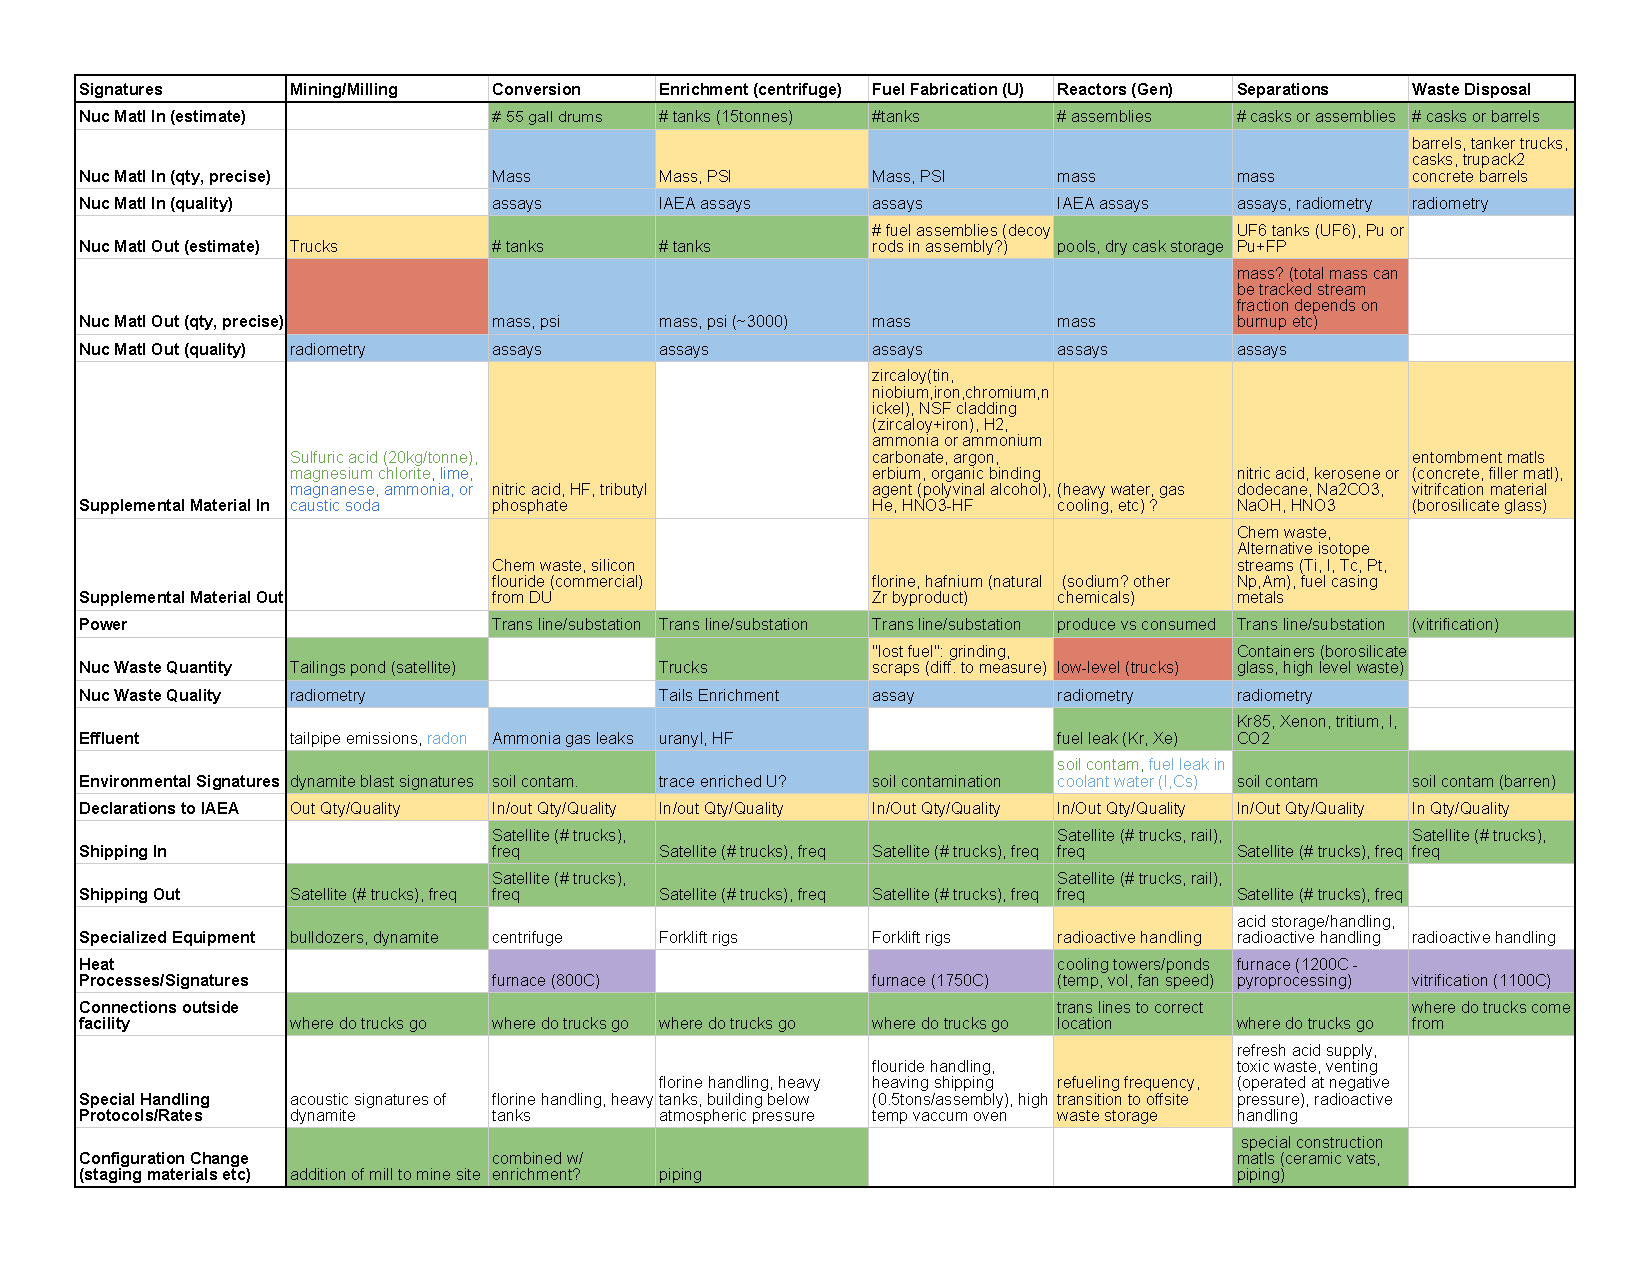
\includegraphics[scale=0.8]{./figs/signatures_table.pdf}
\end{center}
\caption{Table of potential signatures across the fuel cycle: measureable through open, independent sources such as satellite imagery (green), available through official inspections (blue), or potentially unreliable due to physical or political constraints (yellow)\cite{kemp_environmental_2016,_plutonium_????,ferreira_radiometric_2012,stork_systematic_2006}.}
\label{fig:signatures}
\end{figure}
\fi

